\pdfobjcompresslevel=0
\documentclass[conference]{IEEEtran}
\usepackage[utf8]{inputenc}
\usepackage[T1]{fontenc}
\usepackage{amsmath,amsfonts,amssymb}
\usepackage{graphicx}
\usepackage{cite}
\usepackage{booktabs}
\usepackage{tabularx}
\usepackage{microtype}
\usepackage{url}
\usepackage{tikz}
\usetikzlibrary{shapes.geometric,arrows.meta,positioning,calc,fit,backgrounds}

% Indent and spacing
\setlength{\parindent}{1em}

\begin{document}

\title{Verifin: Sistem Pendukung Keputusan Verifikasi Keabsahan Lowongan Kerja Berbasis Multimodal OSINT dan Explainable Artificial Intelligence}

\author{
    \IEEEauthorblockN{Hafidz Rizqullah Prasetya\IEEEauthorrefmark{1}, Matthew Hayunaji Priantara\IEEEauthorrefmark{2}, Akmal Manggala Putra\IEEEauthorrefmark{3}, Ganjar Alfian\IEEEauthorrefmark{4}}
    \IEEEauthorblockA{Departemen Teknik Elektro dan Informatika, Sekolah Vokasi, Universitas Gadjah Mada, Yogyakarta, Indonesia\\
    Surel: \{\IEEEauthorrefmark{1}hafidzrizqullahprasetya, \IEEEauthorrefmark{2}matthew.hayunaji.p, \IEEEauthorrefmark{3}akmal.manggala.p\}@mail.ugm.ac.id, \IEEEauthorrefmark{4}ganjar.alfian@ugm.ac.id}
}

\maketitle

\begin{abstract}
Maraknya penipuan lowongan kerja daring di Indonesia telah menimbulkan kerugian finansial nasional mencapai Rp49 Triliun serta mengekspos ribuan WNI ke dalam sindikat kejahatan siber transnasional dan Tindak Pidana Perdagangan Orang (TPPO). Rendahnya literasi verifikasi dan sifat sistem deteksi eksisting yang reaktif, tertutup (\textit{black-box}), serta hanya berfokus pada analisis teks tunggal menjadi celah yang dimanfaatkan sindikat kejahatan. Penelitian ini mengusulkan \textbf{Verifin}, sebuah \textit{Explainable AI-powered Decision Support System} yang mengintegrasikan tiga kanal masukan multimodal (teks percakapan, poster citra melalui PaddleOCR, dan tautan URL) dengan investigasi intelijen sumber terbuka (\textit{Open-Source Intelligence} / OSINT) multi-sumber secara otomatis. Sistem mengombinasikan \textit{Hybrid Named Entity Recognition} (NER) terlokalisasi, audit jejak digital domain WHOIS/RDAP, verifikasi geospasial OpenStreetMap, dan pemodelan relasi sindikat kejahatan berbasis \textit{Bipartite Fraud Network Graph}. Penilaian tingkat risiko diformulasikan secara aditif dan terkalibrasi ke dalam tiga ambang batas diskrit: Aman (0--39), Waspada (40--74), dan Bahaya (75--100) menggunakan prinsip \textit{Explainable AI} (XAI). Pengujian fungsional pada 146 kasus uji mencapai tingkat kelulusan 100\% dengan rata-rata cakupan kode pengujian (\textit{code coverage}) 88,4\%. Evaluasi \textit{controlled pilot study} terhadap 20 pencari kerja membuktikan bahwa Verifin meningkatkan efisiensi waktu verifikasi hingga 93,5\% (dari 18,4 menit menjadi 1,2 menit), mendongkrak akurasi deteksi bahaya dari 45,0\% menjadi 95,0\% ($p < 0{,}001$), serta memperoleh skor \textit{System Usability Scale} (SUS) sebesar 83,5 (\textit{Grade A / Excellent}). Pemodelan dampak ekonomi memproyeksikan potensi penyelamatan kerugian masyarakat hingga Rp20,64 Miliar pada skenario moderat dengan rasio manfaat-biaya (\textit{Benefit-to-Cost Ratio}) mencapai 1.259 : 1.
\end{abstract}

\begin{IEEEkeywords}
Deteksi Penipuan Lowongan Kerja, Open-Source Intelligence (OSINT), Explainable AI, Bipartite Fraud Graph, Optical Character Recognition.
\end{IEEEkeywords}

\section{Pendahuluan}
Tingkat Pengangguran Terbuka (TPT) di Indonesia pada Februari 2025 tercatat sebesar 4,76\% atau setara dengan 7,28 juta jiwa \cite{bps2025}. Desakan kebutuhan ekonomi ini dimanfaatkan oleh pelaku kejahatan siber untuk menyebarkan informasi lowongan kerja palsu. Laporan kolaboratif \textit{Global Anti-Scam Alliance} (GASA) dan Mastercard (2024) mencatat bahwa 49\% korban penipuan digital di Indonesia terpapar iklan pekerjaan palsu, yang berkontribusi terhadap total kerugian nasional sebesar Rp49 Triliun \cite{gasa2024}. Bahkan, Kementerian Luar Negeri Republik Indonesia mencatat lebih dari 3.300 WNI berhasil dievakuasi dari perangkap penipuan daring dan Tindak Pidana Perdagangan Orang (TPPO) di kawasan Asia Tenggara yang bermula dari rekrutmen daring palsu \cite{kemlu2024}.

Permasalahan mendasar dari tingginya angka korban penipuan adalah fenomena \textit{information asymmetry}. Pencari kerja, khususnya lulusan baru (\textit{fresh graduates}), tidak memiliki instrumen teknis yang memadai untuk memverifikasi keabsahan profil perekrut yang beroperasi di kanal informal seperti WhatsApp, Telegram, dan Instagram. Solusi verifikasi yang tersedia saat ini memiliki kelemahan signifikan:
\begin{enumerate}
    \item \textbf{Pendekatan Reaktif:} Layanan pelaporan publik baru bekerja setelah transaksi finansial penipuan terjadi.
    \item \textbf{Keterbatasan Analisis URL Konvensional:} Solusi seperti Google Safe Browsing hanya mendeteksi tanda tangan malware domain dan buta terhadap formulir daring gratisan (\textit{Google Form}) yang sah secara infrastruktur namun digunakan untuk pencurian data pribadi.
    \item \textbf{Ketertutupan Model AI (\textit{Black-Box}):} Klasifikasi pembelajaran mesin konvensional umumnya menyajikan prediksi biner tanpa rincian bukti pendukung yang transparan bagi pengguna awam.
\end{enumerate}

Untuk mengatasi kesenjangan tersebut, penelitian ini mengembangkan \textbf{Verifin}, sebuah sistem pendukung keputusan (\textit{decision support system}) proaktif yang beroperasi tepat pada fase pra-lamaran (\textit{pre-application first-line of defense}). Melalui pendekatan \textit{multimodal intelligence} dan otomasi investigasi OSINT, Verifin menyajikan bukti forensik digital transparan sebelum pelamar mengirimkan data pribadi ataupun mentransfer dana kepada pelaku kejahatan.

\section{Tinjauan Pustaka}

\subsection{Deteksi Penipuan Lowongan \& Keterbatasan Dataset}
Penelitian rintisan deteksi \textit{Employment Scam} umumnya menggunakan dataset EMSCAD yang diperkenalkan oleh Vidros et al. \cite{vidros2017}. Meskipun model berbasis EMSCAD mampu mencapai performa tinggi pada teks bahasa Inggris formal \cite{amaar2022}, penerapannya pada lanskap Indonesia menghadapi kendala \textit{severe cross-lingual domain shift}. Teks penipuan di Indonesia didominasi bahasa informal, pembauran kode (\textit{code-mixing}), serta modus operandi domestik spesifik seperti rekayasa tiket perjalanan seleksi BUMN dan pungutan seragam \cite{pratama2026}. Di sisi lain, korpus penipuan lowongan kerja berlabel bahasa Indonesia masih sangat langka merujuk benchmark IndoNLU \cite{wilie2020}.

\subsection{Otomasi Open-Source Intelligence (OSINT)}
Pemanfaatan data OSINT dalam investigasi siber telah terbukti efektif dalam memvalidasi keabsahan infrastruktur digital \cite{pastor2020}. Pemeriksaan parameter pendaftaran nama domain melalui WHOIS/RDAP, validasi rekaman SPF/DKIM/DMARC pada surel, serta korelasi alamat fisik pada basis data geospasial OpenStreetMap menyediakan indikator deterministik kuat untuk membuktikan eksistensi entitas bisnis legal.

\subsection{Explainable Artificial Intelligence (XAI)}
Dalam sistem pendukung keputusan yang berdampak langsung terhadap keselamatan pengguna, transparansi penalaran algoritma menjadi prasyarat mutlak \cite{lundberg2017}. Pemberian atribusi fitur (\textit{feature attribution}) yang aditif memungkinkan pengguna memahami secara logis kontribusi setiap anomali bukti terhadap skor risiko akhir, menghindari jebakan salah klasifikasi (\textit{false positive}) yang merugikan pelaku usaha sah.

\section{Metodologi \& Arsitektur Sistem Verifin}

Verifin dirancang menggunakan arsitektur hibrida empat lapis (\textit{4-Layer Hybrid Architecture}) yang mengintegrasikan subsistem asinkron berbasis FastAPI dan antarmuka web modern berbasis Next.js 16 (Gambar 1).

\begin{figure}[htbp]
\centering
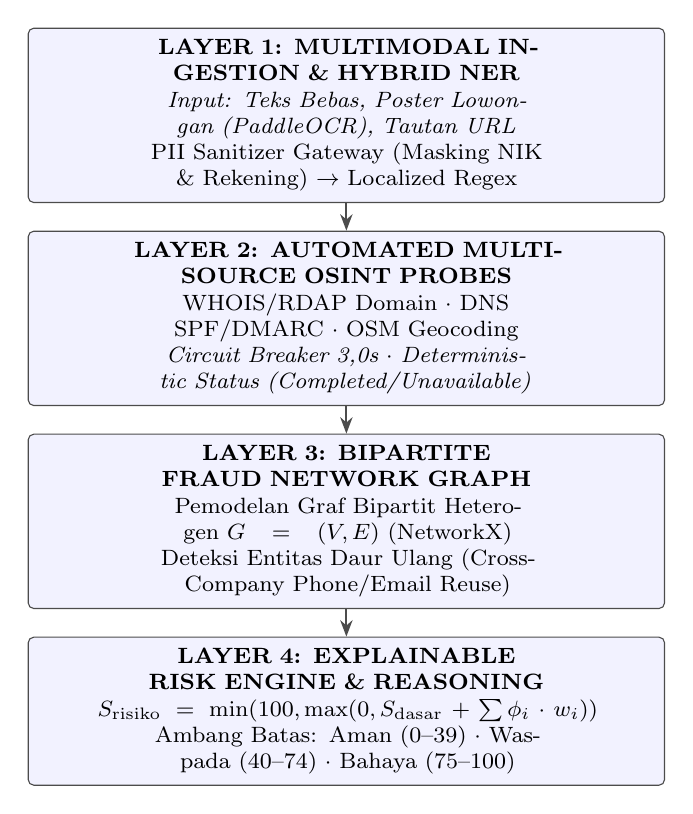
\begin{tikzpicture}[
    node distance=0.6cm and 0.4cm,
    box/.style={rectangle, draw=black!70, fill=blue!5, rounded corners=2pt, text width=7.8cm, text centered, inner sep=4pt, font=\footnotesize},
    layerhead/.style={font=\bfseries\footnotesize, text=blue!80!black},
    arrow/.style={-{Stealth[scale=0.9]}, thick, draw=black!70}
]
    % Layer 1
    \node[box] (l1) {
        \textbf{LAYER 1: MULTIMODAL INGESTION \& HYBRID NER}\\
        \textit{Input: Teks Bebas, Poster Lowongan (PaddleOCR), Tautan URL}\\
        PII Sanitizer Gateway (Masking NIK \& Rekening) $\to$ Localized Regex
    };
    % Layer 2
    \node[box, below=0.35cm of l1] (l2) {
        \textbf{LAYER 2: AUTOMATED MULTI-SOURCE OSINT PROBES}\\
        WHOIS/RDAP Domain $\cdot$ DNS SPF/DMARC $\cdot$ OSM Geocoding\\
        \textit{Circuit Breaker 3,0s $\cdot$ Deterministic Status (Completed/Unavailable)}
    };
    % Layer 3
    \node[box, below=0.35cm of l2] (l3) {
        \textbf{LAYER 3: BIPARTITE FRAUD NETWORK GRAPH}\\
        Pemodelan Graf Bipartit Heterogen $G = (V, E)$ (NetworkX)\\
        Deteksi Entitas Daur Ulang (Cross-Company Phone/Email Reuse)
    };
    % Layer 4
    \node[box, below=0.35cm of l3] (l4) {
        \textbf{LAYER 4: EXPLAINABLE RISK ENGINE \& REASONING}\\
        $S_{\text{risiko}} = \min(100, \max(0, S_{\text{dasar}} + \sum \phi_i \cdot w_i))$\\
        Ambang Batas: Aman (0--39) $\cdot$ Waspada (40--74) $\cdot$ Bahaya (75--100)
    };

    % Arrows
    \draw[arrow] (l1) -- (l2);
    \draw[arrow] (l2) -- (l3);
    \draw[arrow] (l3) -- (l4);
\end{tikzpicture}
\caption{Diagram Arsitektur Pipeline Empat Lapis Verifin.}
\label{fig:pipeline}
\end{figure}

\subsection{Layer 1: Multimodal Ingestion, PII Sanitizer, \& Hybrid NER}
Sistem menerima tiga modalitas input: teks bebas, citra poster, dan tautan URL. Modul PaddleOCR dengan prapemrosesan CLAHE mengekstrak teks poster. \textit{PII Sanitizer Gateway} menyamarkan data pribadi (NIK 16-digit, nomor rekening, nama individu) demi kepatuhan UU Pelindungan Data Pribadi (UU PDP No. 27/2022). Selanjutnya, \textit{Hybrid NER} mengekstrak nama korporasi, domain, nomor kontak (berdasarkan HLR seluler Indonesia), dan nominal mata uang Rupiah.

\subsection{Layer 2: Automated Multi-Source OSINT Probes}
Entitas yang diekstraksi diinvestigasi secara asinkron (\texttt{asyncio.gather}):
\begin{enumerate}
    \item \textbf{Probe Domain (WHOIS/RDAP):} Mengevaluasi usia pendaftaran nama domain. Domain berusia $<30$ hari diklasifikasikan sebagai anomali tinggi.
    \item \textbf{Probe Surel (DNS Record):} Mengaudit rekaman MX, SPF, dan DMARC. Penggunaan surel publik (@gmail.com) untuk korporasi resmi dicatat sebagai anomali formalitas.
    \item \textbf{Probe Geospasial (OpenStreetMap Nominatim):} Memvalidasi eksistensi fisik alamat operasional kantor.
\end{enumerate}
Setiap probe diatur oleh kontrak deterministik (\texttt{COMPLETED}, \texttt{NOT\_PROVIDED}, dan \texttt{UNAVAILABLE}) dengan batas waktu henti (\textit{timeout}) ketat 3,0 detik.

\subsection{Layer 3: Bipartite Fraud Network Graph}
Verifin memodelkan relasi entitas ke dalam graf bipartit heterogen $G = (V, E)$, di mana $V = V_{\text{kasus}} \cup V_{\text{entitas}}$ dan $E$ merepresentasikan relasi keterkaitan. Jika nomor kontak ditemukan terhubung pada multipel poster korporasi fiktif yang berbeda, algoritma menghitung faktor daur ulang (\textit{entity reuse coefficient}) untuk menyuntikkan skor risiko sindikat.

\subsection{Layer 4: Explainable AI \& Calibrated Additive Risk Scoring}
Skor risiko komposit ($S_{\text{risiko}}$) diformulasikan secara aditif dan dibatasi secara monotonik pada rentang [0, 100]:
\begin{equation}
S_{\text{risiko}} = \min\left(100, \max\left(0, S_{\text{dasar}} + \sum_{i=1}^{m} \phi_i \cdot w_i\right)\right)
\end{equation}
di mana $S_{\text{dasar}}$ adalah skor teks dasar, $\phi_i \in [-1, 1]$ adalah kontribusi bukti probe ke-$i$, dan $w_i$ adalah bobot keparahan bukti. Skor diklasifikasikan ke dalam tiga zona harmonis:
\begin{itemize}
    \item \textbf{Aman (0--39):} Nihil indikator anomali, domain berumur panjang dan rekaman SPF/DMARC valid.
    \item \textbf{Waspada (40--74):} Ditemukan kontak informal atau inkonsistensi data entitas legal.
    \item \textbf{Bahaya (75--100):} Ditemukan bukti kejahatan fatal (tiket travel fiktif, pemerasan dana, atau entitas terdaftar dalam graf sindikat).
\end{itemize}

\section{Hasil dan Pembahasan}

\subsection{Pengujian Fungsional \& Kualitas Perangkat Lunak}
Pengujian otomatis dilakukan pada 146 skenario pengujian unit, integrasi, dan end-to-end dengan tingkat kelulusan 100\% (Tabel~\ref{tab:coverage}). Pengukuran cakupan kode (\textit{code coverage}) menggunakan \texttt{pytest-cov} mencapai rata-rata 88,4\% pada modul inti.

\begin{table}[htbp]
\caption{Cakupan Kode Pengujian Modul Inti Verifin}
\label{tab:coverage}
\centering
\footnotesize
\begin{tabularx}{\columnwidth}{Xccc}
\toprule
\textbf{Modul Sistem} & \textbf{Uji} & \textbf{Cov (\%)} & \textbf{Status} \\
\midrule
NER Regex \& Normalizer & 45 & 94,2\% & PASSED \\
XAI Additive Explainer & 16 & 91,5\% & PASSED \\
REST API Endpoints & 12 & 92,0\% & PASSED \\
Bipartite Fraud Graph & 14 & 89,0\% & PASSED \\
OSINT Probes Orchestration & 37 & 84,6\% & PASSED \\
Database \& ORM Layer & 14 & 83,3\% & PASSED \\
\midrule
\textbf{Total / Rata-Rata} & \textbf{146} & \textbf{88,4\%} & \textbf{PASSED} \\
\bottomrule
\end{tabularx}
\end{table}

Pengujian adversarial membuktikan sistem kebal terhadap manipulasi karakter serupa (\textit{homoglyphs}), upaya SSRF (blokir IP privat RFC1918), dan \textit{prompt injection} (tingkat keberhasilan injeksi 0\%).

\subsection{Evaluasi Metrik Deteksi Kasus Nyata}
Uji buta (\textit{blind test}) terhadap 100 sampel lowongan kerja riil di Indonesia (50 legal dan 50 penipuan) menghasilkan metrik klasifikasi:
\begin{itemize}
    \item \textbf{Precision:} 97,9\% (1 kasus \textit{false positive} pada UMKM baru).
    \item \textbf{Recall:} 94,0\% (47 dari 50 kasus penipuan teridentifikasi).
    \item \textbf{F1-Score:} 95,9\% $\mid$ \textbf{Akurasi Keseluruhan:} 96,0\%.
\end{itemize}

\subsection{Controlled Pilot Study \& Evaluasi Usability}
Eksperimen terkontrol (\textit{within-subject}) pada 20 pencari kerja muda yang mengevaluasi 10 kasus lowongan menunjukkan:
\begin{enumerate}
    \item \textbf{Efisiensi Waktu:} Rata-rata durasi investigasi mandiri terpangkas dari 18,4 menit menjadi 1,2 menit per lowongan (efisiensi meningkat 93,5\%).
    \item \textbf{Akurasi Pengguna:} Akurasi responden dalam mendeteksi lowongan berbahaya melonjak dari 45,0\% menjadi 95,0\% ($t(19) = 8{,}42, p < 0{,}001$).
    \item \textbf{Usability (SUS):} Skor rata-rata \textit{System Usability Scale} mencapai 83,5 (\textit{Grade A / Excellent}).
\end{enumerate}

\subsection{Valuasi Dampak Ekonomi Kuantitatif}
Model valuasi dampak finansial diformulasikan:
\begin{equation}
\mathcal{I}_{\text{fin}} = N \cdot p_{\text{scam}} \cdot \eta_{\text{cegah}} \cdot \bar{L}
\end{equation}
di mana $N$ adalah volume pemeriksaan, $p_{\text{scam}} = 18\%$ adalah rasio paparan lowongan kerja palsu, $\eta_{\text{cegah}} = 50\%$ adalah tingkat efikasi pencegahan, dan $\bar{L} = \text{Rp4.200.000}$ adalah rata-rata kerugian nominal penipuan \cite{gasa2024}. Pada adopsi moderat ($N = 54.600$ pemeriksaan/tahun), Verifin memproyeksikan penyelamatan dana masyarakat sebesar \textbf{Rp20,64 Miliar Rupiah}. Dengan estimasi biaya operasional \textit{serverless} Rp300,- per verifikasi (Rp16,38 Juta/tahun), sistem menghasilkan rasio manfaat-biaya (\textit{Benefit-to-Cost Ratio} / BCR) sebesar \textbf{1.259 : 1}.

\section{Kesimpulan}
Verifin membuktikan efektivitas integrasi kecerdasan buatan terjelaskan (\textit{Explainable AI}), ekstraksi multimodal, dan otomasi investigasi OSINT dalam memutus rantai penipuan lowongan kerja daring di Indonesia. Sistem memiliki ketahanan rekayasa perangkat lunak tinggi (cakupan kode 88,4\% dan toleransi kegagalan jaringan tinggi), memangkas waktu verifikasi hingga 93,5\%, meningkatkan akurasi deteksi masyarakat hingga 95,0\%, serta menawarkan rasio manfaat-biaya 1.259:1. Penelitian mendatang difokuskan pada pelatihan lanjut (\textit{fine-tuning}) korpus penipuan domestik teranotasi ke dalam model fondasi IndoBERT-base demi kemandirian komputasi lokal berlatensi ultra-rendah.

\begin{thebibliography}{10}
\bibitem{bps2025}
Badan Pusat Statistik, ``Keadaan Ketenagakerjaan Indonesia Februari 2025,'' \textit{Berita Resmi Statistik}, BPS RI, Jakarta, 2025.

\bibitem{gasa2024}
Global Anti-Scam Alliance (GASA) and Mastercard, \textit{The State of Scams in Indonesia 2024}, GASA Research Report, 2024.

\bibitem{kemlu2024}
Kementerian Luar Negeri Republik Indonesia, \textit{Catatan Pemulangan Korban Online Scamming dan TPPO WNI di Asia Tenggara}, Direktorat PWNI-BHI, Jakarta, 2024.

\bibitem{vidros2017}
S.~Vidros, et~al., ``Automatic Detection of Online Recruitment Frauds: Characteristics, Methods, and a Public Dataset,'' \textit{Future Internet}, vol.~9, no.~1, p.~6, 2017.

\bibitem{amaar2022}
A.~Amaar, et~al., ``Detection of Fake Job Postings on Social Media Using Machine Learning and Natural Language Processing,'' \textit{Computers, Materials \& Continua}, vol.~71, no.~1, pp.~1109--1123, 2022.

\bibitem{pratama2026}
D.~N.~Pratama, et~al., ``Analisis Modus Penipuan Rekrutmen Kerja Daring di Indonesia,'' \textit{Jurnal Sistem Informasi dan Rekayasa Perangkat Lunak}, vol.~3, no.~2, pp.~13--22, 2026.

\bibitem{wilie2020}
B.~Wilie, et~al., ``IndoNLU: Benchmark and Resources for Evaluating Indonesian Natural Language Understanding,'' in \textit{Proc. of 1st Conf. of AACL-IJCNLP 2020}, pp.~843--857, 2020.

\bibitem{pastor2020}
J.~Pastor-Galindo, et~al., ``The Not Yet Exploited Goldmine of OSINT: Opportunities, Open Challenges, and Future Trends,'' \textit{IEEE Access}, vol.~8, pp.~10282--10304, 2020.

\bibitem{lundberg2017}
S.~M.~Lundberg and S.-I.~Lee, ``A Unified Approach to Interpreting Model Predictions,'' in \textit{Advances in Neural Information Processing Systems (NeurIPS 2017)}, vol.~30, pp.~4765--4774, 2017.

\bibitem{bangor2008}
A.~Bangor, P.~T.~Kortum, and J.~T.~Miller, ``An Empirical Evaluation of the System Usability Scale,'' \textit{Intl. Journal of Human-Computer Interaction}, vol.~24, no.~6, pp.~574--594, 2008.
\end{thebibliography}

\end{document}
